% Options for packages loaded elsewhere
\PassOptionsToPackage{unicode}{hyperref}
\PassOptionsToPackage{hyphens}{url}
\documentclass[
]{article}
\usepackage{xcolor}
\usepackage[margin=1in]{geometry}
\usepackage{amsmath,amssymb}
\setcounter{secnumdepth}{5}
\usepackage{iftex}
\ifPDFTeX
  \usepackage[T1]{fontenc}
  \usepackage[utf8]{inputenc}
  \usepackage{textcomp} % provide euro and other symbols
\else % if luatex or xetex
  \usepackage{unicode-math} % this also loads fontspec
  \defaultfontfeatures{Scale=MatchLowercase}
  \defaultfontfeatures[\rmfamily]{Ligatures=TeX,Scale=1}
\fi
\usepackage{lmodern}
\ifPDFTeX\else
  % xetex/luatex font selection
\fi
% Use upquote if available, for straight quotes in verbatim environments
\IfFileExists{upquote.sty}{\usepackage{upquote}}{}
\IfFileExists{microtype.sty}{% use microtype if available
  \usepackage[]{microtype}
  \UseMicrotypeSet[protrusion]{basicmath} % disable protrusion for tt fonts
}{}
\makeatletter
\@ifundefined{KOMAClassName}{% if non-KOMA class
  \IfFileExists{parskip.sty}{%
    \usepackage{parskip}
  }{% else
    \setlength{\parindent}{0pt}
    \setlength{\parskip}{6pt plus 2pt minus 1pt}}
}{% if KOMA class
  \KOMAoptions{parskip=half}}
\makeatother
\usepackage{color}
\usepackage{fancyvrb}
\newcommand{\VerbBar}{|}
\newcommand{\VERB}{\Verb[commandchars=\\\{\}]}
\DefineVerbatimEnvironment{Highlighting}{Verbatim}{commandchars=\\\{\}}
% Add ',fontsize=\small' for more characters per line
\usepackage{framed}
\definecolor{shadecolor}{RGB}{248,248,248}
\newenvironment{Shaded}{\begin{snugshade}}{\end{snugshade}}
\newcommand{\AlertTok}[1]{\textcolor[rgb]{0.94,0.16,0.16}{#1}}
\newcommand{\AnnotationTok}[1]{\textcolor[rgb]{0.56,0.35,0.01}{\textbf{\textit{#1}}}}
\newcommand{\AttributeTok}[1]{\textcolor[rgb]{0.13,0.29,0.53}{#1}}
\newcommand{\BaseNTok}[1]{\textcolor[rgb]{0.00,0.00,0.81}{#1}}
\newcommand{\BuiltInTok}[1]{#1}
\newcommand{\CharTok}[1]{\textcolor[rgb]{0.31,0.60,0.02}{#1}}
\newcommand{\CommentTok}[1]{\textcolor[rgb]{0.56,0.35,0.01}{\textit{#1}}}
\newcommand{\CommentVarTok}[1]{\textcolor[rgb]{0.56,0.35,0.01}{\textbf{\textit{#1}}}}
\newcommand{\ConstantTok}[1]{\textcolor[rgb]{0.56,0.35,0.01}{#1}}
\newcommand{\ControlFlowTok}[1]{\textcolor[rgb]{0.13,0.29,0.53}{\textbf{#1}}}
\newcommand{\DataTypeTok}[1]{\textcolor[rgb]{0.13,0.29,0.53}{#1}}
\newcommand{\DecValTok}[1]{\textcolor[rgb]{0.00,0.00,0.81}{#1}}
\newcommand{\DocumentationTok}[1]{\textcolor[rgb]{0.56,0.35,0.01}{\textbf{\textit{#1}}}}
\newcommand{\ErrorTok}[1]{\textcolor[rgb]{0.64,0.00,0.00}{\textbf{#1}}}
\newcommand{\ExtensionTok}[1]{#1}
\newcommand{\FloatTok}[1]{\textcolor[rgb]{0.00,0.00,0.81}{#1}}
\newcommand{\FunctionTok}[1]{\textcolor[rgb]{0.13,0.29,0.53}{\textbf{#1}}}
\newcommand{\ImportTok}[1]{#1}
\newcommand{\InformationTok}[1]{\textcolor[rgb]{0.56,0.35,0.01}{\textbf{\textit{#1}}}}
\newcommand{\KeywordTok}[1]{\textcolor[rgb]{0.13,0.29,0.53}{\textbf{#1}}}
\newcommand{\NormalTok}[1]{#1}
\newcommand{\OperatorTok}[1]{\textcolor[rgb]{0.81,0.36,0.00}{\textbf{#1}}}
\newcommand{\OtherTok}[1]{\textcolor[rgb]{0.56,0.35,0.01}{#1}}
\newcommand{\PreprocessorTok}[1]{\textcolor[rgb]{0.56,0.35,0.01}{\textit{#1}}}
\newcommand{\RegionMarkerTok}[1]{#1}
\newcommand{\SpecialCharTok}[1]{\textcolor[rgb]{0.81,0.36,0.00}{\textbf{#1}}}
\newcommand{\SpecialStringTok}[1]{\textcolor[rgb]{0.31,0.60,0.02}{#1}}
\newcommand{\StringTok}[1]{\textcolor[rgb]{0.31,0.60,0.02}{#1}}
\newcommand{\VariableTok}[1]{\textcolor[rgb]{0.00,0.00,0.00}{#1}}
\newcommand{\VerbatimStringTok}[1]{\textcolor[rgb]{0.31,0.60,0.02}{#1}}
\newcommand{\WarningTok}[1]{\textcolor[rgb]{0.56,0.35,0.01}{\textbf{\textit{#1}}}}
\usepackage{longtable,booktabs,array}
\usepackage{calc} % for calculating minipage widths
% Correct order of tables after \paragraph or \subparagraph
\usepackage{etoolbox}
\makeatletter
\patchcmd\longtable{\par}{\if@noskipsec\mbox{}\fi\par}{}{}
\makeatother
% Allow footnotes in longtable head/foot
\IfFileExists{footnotehyper.sty}{\usepackage{footnotehyper}}{\usepackage{footnote}}
\makesavenoteenv{longtable}
\usepackage{graphicx}
\makeatletter
\newsavebox\pandoc@box
\newcommand*\pandocbounded[1]{% scales image to fit in text height/width
  \sbox\pandoc@box{#1}%
  \Gscale@div\@tempa{\textheight}{\dimexpr\ht\pandoc@box+\dp\pandoc@box\relax}%
  \Gscale@div\@tempb{\linewidth}{\wd\pandoc@box}%
  \ifdim\@tempb\p@<\@tempa\p@\let\@tempa\@tempb\fi% select the smaller of both
  \ifdim\@tempa\p@<\p@\scalebox{\@tempa}{\usebox\pandoc@box}%
  \else\usebox{\pandoc@box}%
  \fi%
}
% Set default figure placement to htbp
\def\fps@figure{htbp}
\makeatother
\setlength{\emergencystretch}{3em} % prevent overfull lines
\providecommand{\tightlist}{%
  \setlength{\itemsep}{0pt}\setlength{\parskip}{0pt}}
\usepackage{pdfpages}
\usepackage{tcolorbox}
\usepackage{graphicx}
\usepackage{setspace}
\usepackage{bookmark}
\IfFileExists{xurl.sty}{\usepackage{xurl}}{} % add URL line breaks if available
\urlstyle{same}
\hypersetup{
  hidelinks,
  pdfcreator={LaTeX via pandoc}}

\author{}
\date{\vspace{-2.5em}}

\begin{document}


\includepdf{Page_de_garde}

\newpage

\setstretch{1}

\renewcommand{\contentsname}{\textcolor{blue}{Sommaire}}

\textcolor{blue}{\tableofcontents}

\newpage

\begin{tcolorbox}[colback=white,colframe=blue, title=Avant-propos ]

Créée en 2008, l’École Nationale de la Statistique et de l’Analyse Économique (ENSAE) est une grande école de statistique à caractère sous-régional située à Dakar (capitale du Sénégal). Elle constitue une direction de l’Agence Nationale de la Statistique et de la Démographie (ANSD), qui est la structure principale du Système Statistique Nationale du Sénégal. 


  Les élèves Ingénieurs Statisticiens Economistes qui suivent une formation de ISE (03 ans pour le cycle court et 05 ans pour le cycle long) à l'ENSAE  se doivent de suivre le module \textcolor{blue}{Projet statistique sous R } pour apprendre à utiliser et à traiter les données statistiques avec ce logiciel et à synthétiser les données à travers des graphiques afin de faciliter leur comprehension. 
  
  
  
\end{tcolorbox}

\newpage

\textcolor{blue}{\section*{INTRODUCTION}\addcontentsline{toc}{section}{INTRODUCTION}}

À l'ère du numérique, la visualisation interactive des données est
devenue un levier incontournable pour la prise de décision. Que ce soit
dans les entreprises, les institutions publiques ou les milieux
académiques, la capacité à transformer des données brutes en
informations exploitables est un atout stratégique majeur. C'est dans ce
contexte que R Shiny s'impose comme une solution puissante et accessible
pour concevoir des tableaux de bord dynamiques et interactifs.

R Shiny, développé par la communauté R, permet de créer facilement des
applications web sans pour autant recourir à des langages comme HTML,
CSS ou JavaScript. Grâce à son interface intuitive, il offre aux
analystes et data scientists la possibilité de déployer rapidement des
outils de visualisation sur mesure, tout en exploitant pleinement
l'écosystème R pour l'analyse de données.

Ce document a pour objectif de présenter les fondamentaux de la création
de tableaux de bord avec R Shiny, d'en illustrer les avantages à travers
des exemples concrets, et de fournir les bonnes pratiques pour
construire des interfaces efficaces et esthétiques.

\newpage

\section{Chargement des packages
nécessaires}\label{chargement-des-packages-nuxe9cessaires}

Avant toute chose, nous veillerons à installer tous les packages qui
servirons dans la suite puis les charger.

\begin{Shaded}
\begin{Highlighting}[]
\NormalTok{packages }\OtherTok{\textless{}{-}} \FunctionTok{c}\NormalTok{(}\StringTok{"tidyverse"}\NormalTok{,}\StringTok{"shiny"}\NormalTok{,}\StringTok{"bslib"}\NormalTok{,}\StringTok{"shinydashboard"}\NormalTok{, }\StringTok{"datasets"}\NormalTok{, }
              \StringTok{"DT"}\NormalTok{, }\StringTok{"rsconnect"}\NormalTok{)}

\ControlFlowTok{for}\NormalTok{ (package }\ControlFlowTok{in}\NormalTok{ packages) \{}
  \ControlFlowTok{if}\NormalTok{ (}\SpecialCharTok{!}\FunctionTok{requireNamespace}\NormalTok{(package, }\AttributeTok{quietly =} \ConstantTok{TRUE}\NormalTok{)) \{}
    \FunctionTok{install.packages}\NormalTok{(package)}
\NormalTok{  \}}
  \FunctionTok{library}\NormalTok{(package, }\AttributeTok{character.only =} \ConstantTok{TRUE}\NormalTok{)}
\NormalTok{\}}
\end{Highlighting}
\end{Shaded}

\begin{itemize}
\tightlist
\item
  Le package \textbf{\texttt{tidyverse}} permet de \textbf{manipuler},
  \textbf{analyser} et \textbf{visualiser} des données de manière
  cohérente grâce à une collection de packages tels que \texttt{dplyr},
  \texttt{ggplot2}, \texttt{tidyr}, entre autres.\\
\item
  Le package \textbf{\texttt{shiny}} permet de \textbf{créer des
  applications web interactives} pour explorer, analyser et visualiser
  des données en temps réel.\\
\item
  Le package \textbf{\texttt{bslib}} permet de \textbf{personnaliser
  facilement l'apparence} d'une application Shiny à l'aide de thèmes
  Bootstrap modernes.\\
\item
  Le package \textbf{\texttt{shinydashboard}} est une extension de Shiny
  qui \textbf{simplifie la création de tableaux de bord interactifs et
  attrayants}.\\
\item
  Le package \textbf{\texttt{datasets}} donne accès à \textbf{divers
  jeux de données standards} (par exemple : \texttt{iris},
  \texttt{mtcars}, \texttt{airquality}, etc.), utiles pour les
  démonstrations et les tests.\\
\item
  Le package \textbf{\texttt{DT}} permet de \textbf{transformer des
  dataframes en tableaux dynamiques et interactifs}, avec des
  fonctionnalités comme le tri, la recherche ou la pagination.\\
\item
  Le package \textbf{\texttt{rsconnect}} permet de \textbf{déployer des
  applications Shiny et des documents R Markdown} sur des serveurs web,
  notamment sur la plateforme
  \href{https://www.shinyapps.io}{shinyapps.io}.
\end{itemize}

\section{Généralités sur R
Shiny}\label{guxe9nuxe9ralituxe9s-sur-r-shiny}

Pour créer une application avec R Shiny, il faut au préalable installer
le package \textcolor{blue}{shiny.}

\subsection{Principes d'une application
Shiny}\label{principes-dune-application-shiny}

Une application \textbf{Shiny} est composée de deux parties essentielles
:\\
\textbf{l'interface utilisateur (UI)} et \textbf{la logique du serveur}.

\begin{itemize}
\tightlist
\item
  L'\textbf{UI} définit la \textbf{mise en page} ainsi que les
  \textbf{éléments interactifs} de l'application (boutons, graphiques,
  menus, etc.).
\item
  Le \textbf{serveur} gère la \textbf{logique métier}, \textbf{traite
  les données} et \textbf{génère les sorties} à afficher à
  l'utilisateur.
\item
  L'interaction entre l'UI et le serveur permet de créer des
  \textbf{applications réactives}, c'est-à-dire capables de répondre
  automatiquement aux actions de l'utilisateur.
\end{itemize}

Pour une meilleure organisation du code, il est recommandé de structurer
l'application Shiny autour d'au moins trois fichiers :

\begin{itemize}
\tightlist
\item
  \textbf{\texttt{ui.R}} : contient le code de l'interface
  utilisateur.\\
\item
  \textbf{\texttt{server.R}} : contient la logique de traitement côté
  serveur.\\
\item
  \textbf{\texttt{app.R}} : combine les deux composants précédents et
  \textbf{lance l'application}.
\end{itemize}

\subsection{Création d'un fichier R
Shiny}\label{cruxe9ation-dun-fichier-r-shiny}

Pour créer un fichier \textbf{R Shiny}, il suffit de suivre les étapes
suivantes :

\begin{itemize}
\tightlist
\item
  Dans la \textbf{barre de menu}, cliquer sur \textbf{File}.\\
\item
  Puis, sélectionner \textbf{New File}, puis \textbf{Shiny Web App}.\\
\item
  Une boîte de dialogue s'affiche :

  \begin{itemize}
  \tightlist
  \item
    Saisir le \textbf{nom de l'application}.\\
  \item
    Choisir le \textbf{type d'application} à créer : un fichier unique
    \texttt{app.R} ou deux fichiers séparés \texttt{ui.R} et
    \texttt{server.R}.\\
  \item
    Préciser le \textbf{répertoire de destination} à l'aide du champ
    \emph{Browse}.\\
  \item
    Cliquer sur \textbf{Create} pour valider.
  \end{itemize}
\end{itemize}

Une fois l'application créée, un \textbf{fichier app.R} s'ouvre
automatiquement dans l'éditeur. Ce fichier contient une structure de
base que nous pouvons adapter à notre projet.

\begin{Shaded}
\begin{Highlighting}[]
\CommentTok{\#}
\CommentTok{\# This is a Shiny web application. You can run the application by clicking}
\CommentTok{\# the \textquotesingle{}Run App\textquotesingle{} button above.}
\CommentTok{\#}
\CommentTok{\# Find out more about building applications with Shiny here:}
\CommentTok{\#}
\CommentTok{\#    https://shiny.posit.co/}
\CommentTok{\#}

\FunctionTok{library}\NormalTok{(shiny)}

\CommentTok{\# Define UI for application that draws a histogram}
\NormalTok{ui }\OtherTok{\textless{}{-}} \FunctionTok{fluidPage}\NormalTok{(}

    \CommentTok{\# Application title}
    \FunctionTok{titlePanel}\NormalTok{(}\StringTok{"Old Faithful Geyser Data"}\NormalTok{),}

    \CommentTok{\# Sidebar with a slider input for number of bins }
    \FunctionTok{sidebarLayout}\NormalTok{(}
        \FunctionTok{sidebarPanel}\NormalTok{(}
            \FunctionTok{sliderInput}\NormalTok{(}\StringTok{"bins"}\NormalTok{,}
                        \StringTok{"Number of bins:"}\NormalTok{,}
                        \AttributeTok{min =} \DecValTok{1}\NormalTok{,}
                        \AttributeTok{max =} \DecValTok{50}\NormalTok{,}
                        \AttributeTok{value =} \DecValTok{30}\NormalTok{)}
\NormalTok{        ),}

        \CommentTok{\# Show a plot of the generated distribution}
        \FunctionTok{mainPanel}\NormalTok{(}
           \FunctionTok{plotOutput}\NormalTok{(}\StringTok{"distPlot"}\NormalTok{)}
\NormalTok{        )}
\NormalTok{    )}
\NormalTok{)}

\CommentTok{\# Define server logic required to draw a histogram}
\NormalTok{server }\OtherTok{\textless{}{-}} \ControlFlowTok{function}\NormalTok{(input, output) \{}

\NormalTok{    output}\SpecialCharTok{$}\NormalTok{distPlot }\OtherTok{\textless{}{-}} \FunctionTok{renderPlot}\NormalTok{(\{}
        \CommentTok{\# generate bins based on input$bins from ui.R}
\NormalTok{        x    }\OtherTok{\textless{}{-}}\NormalTok{ faithful[, }\DecValTok{2}\NormalTok{]}
\NormalTok{        bins }\OtherTok{\textless{}{-}} \FunctionTok{seq}\NormalTok{(}\FunctionTok{min}\NormalTok{(x), }\FunctionTok{max}\NormalTok{(x), }\AttributeTok{length.out =}\NormalTok{ input}\SpecialCharTok{$}\NormalTok{bins }\SpecialCharTok{+} \DecValTok{1}\NormalTok{)}

        \CommentTok{\# draw the histogram with the specified number of bins}
        \FunctionTok{hist}\NormalTok{(x, }\AttributeTok{breaks =}\NormalTok{ bins, }\AttributeTok{col =} \StringTok{\textquotesingle{}darkgray\textquotesingle{}}\NormalTok{, }\AttributeTok{border =} \StringTok{\textquotesingle{}white\textquotesingle{}}\NormalTok{,}
             \AttributeTok{xlab =} \StringTok{\textquotesingle{}Waiting time to next eruption (in mins)\textquotesingle{}}\NormalTok{,}
             \AttributeTok{main =} \StringTok{\textquotesingle{}Histogram of waiting times\textquotesingle{}}\NormalTok{)}
\NormalTok{    \})}
\NormalTok{\}}

\CommentTok{\# Run the application }
\FunctionTok{shinyApp}\NormalTok{(}\AttributeTok{ui =}\NormalTok{ ui, }\AttributeTok{server =}\NormalTok{ server)}
\end{Highlighting}
\end{Shaded}

En compilant ce code nous avons le résultat ci dessous.

\pandocbounded{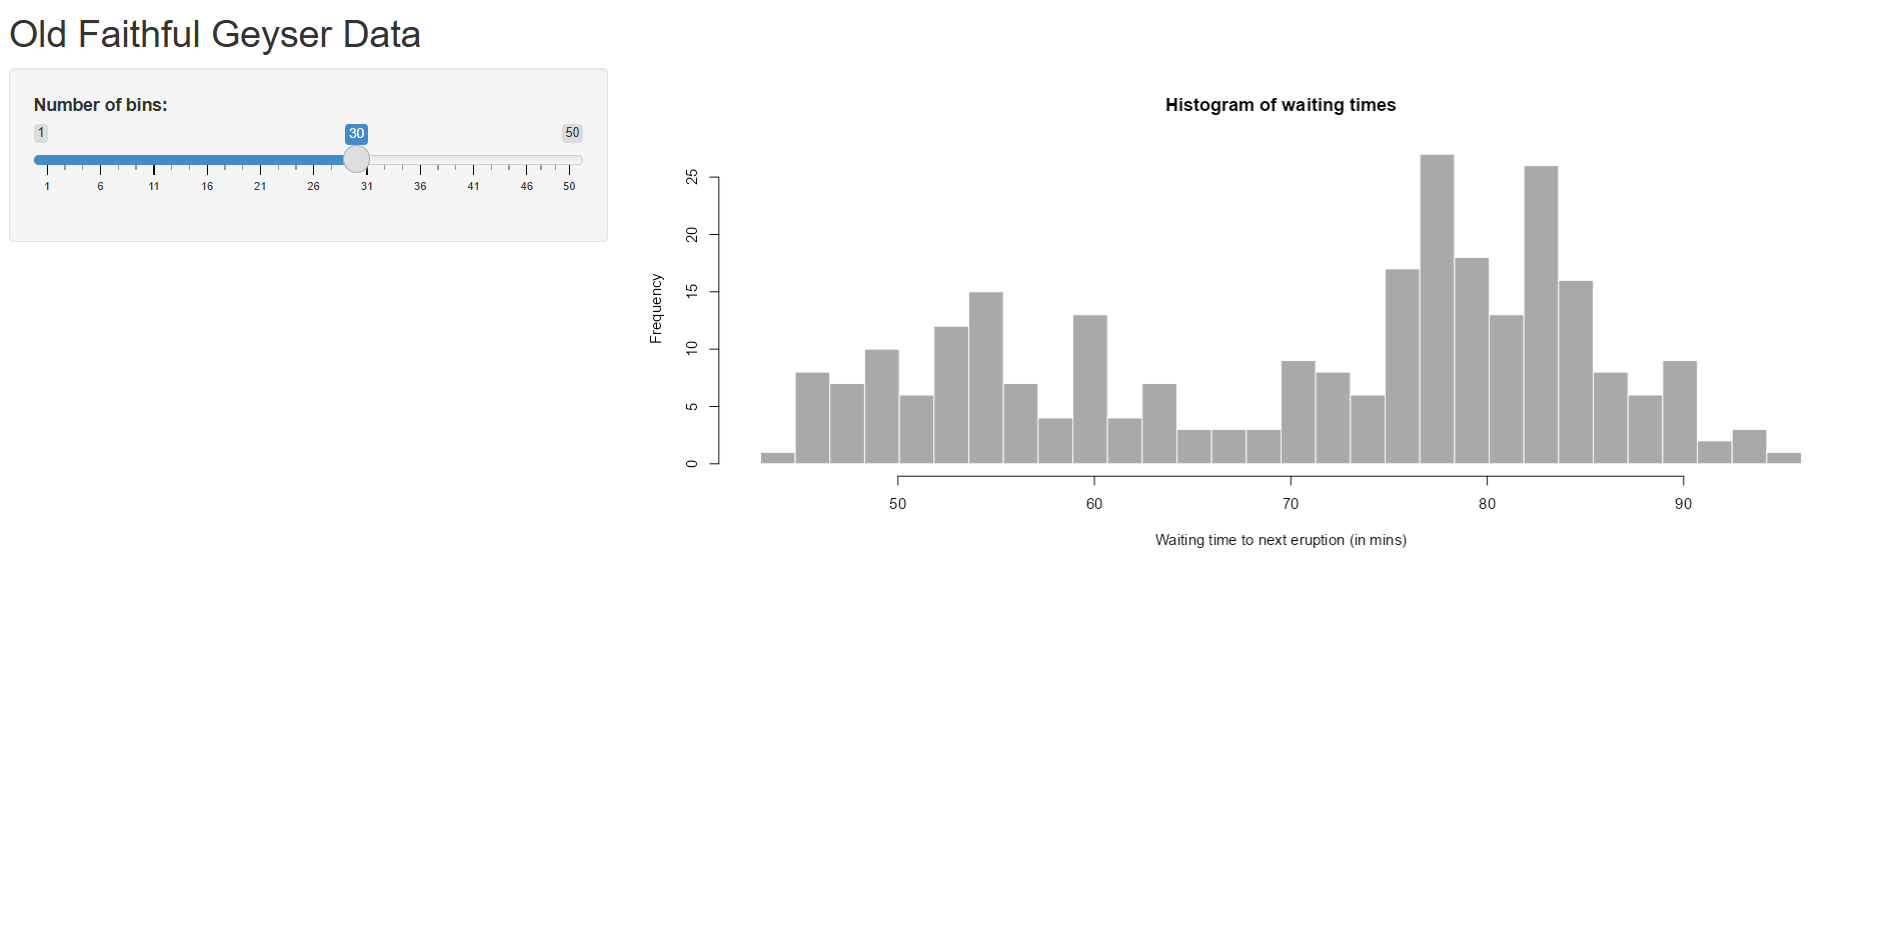
\includegraphics[keepaspectratio]{../images/Base_modele.png}}

\subsection{Parties principales}\label{parties-principales}

Une application Shiny a besoin d'au moins les 4 lignes suivantes :

\begin{Shaded}
\begin{Highlighting}[]
\FunctionTok{library}\NormalTok{(shiny) }\CommentTok{\# Pour le chargement du package Shiny}

\NormalTok{ui }\OtherTok{\textless{}{-}} \FunctionTok{fluidPage}\NormalTok{() }\CommentTok{\#pour la création de l\textquotesingle{}interface utilisateur}

\NormalTok{server }\OtherTok{\textless{}{-}} \ControlFlowTok{function}\NormalTok{(input, output)\{\} }\CommentTok{\#pour la partie serveur}

\FunctionTok{shinyApp}\NormalTok{(ui, server)  }\CommentTok{\# Lancement de l\textquotesingle{}application}
\end{Highlighting}
\end{Shaded}

\begin{Shaded}
\begin{Highlighting}[]
\CommentTok{\#crée l’application avec l’ui et la logique de serveur précédemment créées.}
\end{Highlighting}
\end{Shaded}

Notons que la fonction \textbf{\texttt{fluidPage()}} permet de créer une
page \textbf{Shiny fluide}, qui s'adapte automatiquement à la taille de
la fenêtre du navigateur. Il existe également d'autres types de pages,
comme \textbf{\texttt{fixedPage()}}, qui, contrairement à
\textbf{\texttt{fluidPage()}}, possède une taille fixe et ne s'ajuste
pas à la taille de la fenêtre.

\newpage

\section{Structure d'une application
Shiny}\label{structure-dune-application-shiny}

\subsection{Création de l'interface utilisateur
:}\label{cruxe9ation-de-linterface-utilisateur}

\subsubsection{Les Layouts(dispositions)}\label{les-layoutsdispositions}

Un \textbf{layout} dans R Shiny désigne la \textbf{structure visuelle}
de l'application, c'est-à-dire la manière dont les éléments de
l'interface utilisateur sont organisés à l'écran.

L'interface est généralement construite à partir de \textbf{fonctions
imbriquées}, selon la logique suivante :

\begin{enumerate}
\def\labelenumi{\arabic{enumi}.}
\tightlist
\item
  Une fonction définissant la \textbf{disposition générale}, comme
  \texttt{fluidPage()} (la plus courante).\\
\item
  Des \textbf{panneaux de mise en page} tels que
  \texttt{sidebarPanel()}, \texttt{mainPanel()} ou \texttt{tabPanel()}
  pour organiser le contenu.\\
\item
  Pour créer des onglets, on utilise les fonctions
  \texttt{tabsetPanel()} (disposition horizontale) ou
  \texttt{navlistPanel()} (disposition verticale), afin de diviser
  l'affichage en plusieurs sections indépendantes.
\end{enumerate}

\begin{Shaded}
\begin{Highlighting}[]
\FunctionTok{library}\NormalTok{(shiny)}


\NormalTok{ui }\OtherTok{\textless{}{-}} \FunctionTok{fluidPage}\NormalTok{(}
  \FunctionTok{titlePanel}\NormalTok{(}\StringTok{"Notre application Shiny"}\NormalTok{),}

  \FunctionTok{sidebarLayout}\NormalTok{(}
    \FunctionTok{sidebarPanel}\NormalTok{(}\StringTok{"Panneau latéral"}\NormalTok{),}
    \FunctionTok{mainPanel}\NormalTok{(}
      \FunctionTok{tabsetPanel}\NormalTok{(}
        \FunctionTok{tabPanel}\NormalTok{(}\StringTok{"Onglet 1"}\NormalTok{, }\StringTok{"Contenu de l\textquotesingle{}onglet 1"}\NormalTok{),}
        \FunctionTok{tabPanel}\NormalTok{(}\StringTok{"Onglet 2"}\NormalTok{, }\StringTok{"Contenu de l\textquotesingle{}onglet 2"}\NormalTok{)}
\NormalTok{      )}
\NormalTok{    )}
\NormalTok{  )}
\NormalTok{)}
\CommentTok{\# Run the application }
\FunctionTok{shinyApp}\NormalTok{(}\AttributeTok{ui =}\NormalTok{ ui, }\AttributeTok{server =}\NormalTok{ server)}
\end{Highlighting}
\end{Shaded}

Voici comment se présentent la disposition horizontale :

\pandocbounded{
\includegraphics[keepaspectratio]{../images/dispo.png}}

\subsubsection{Autres dispositions
possibles}\label{autres-dispositions-possibles}

Shiny offre plusieurs fonctions pour créer des interfaces variées :

\begin{itemize}
\tightlist
\item
  \textbf{\texttt{navbarPage()}} : permet d'ajouter une \textbf{barre de
  navigation horizontale} en haut de l'application.\\
\item
  \textbf{\texttt{navbarMenu()}} : permet de \textbf{regrouper plusieurs
  \texttt{tabPanel()}} sous un même menu déroulant.\\
\item
  \textbf{\texttt{column()}} : permet de \textbf{disposer des éléments
  en colonnes}, utile pour créer des mises en page personnalisées.
\end{itemize}

\textbf{À noter :} Les packages \textbf{\texttt{bslib}} et
\textbf{\texttt{shinydashboard}} offrent encore plus de flexibilité pour
créer des interfaces modernes et structurées, grâce à leurs propres
fonctions de mise en page.

\subsection{Inputs-Outputs}\label{inputs-outputs}

\subsubsection{Inputs (widgets)}\label{inputs-widgets}

Les \textbf{inputs} permettent aux utilisateurs d'interagir avec
l'application. Ils sont généralement placés dans le
\textbf{\texttt{sidebarPanel()}}.

Parmi les plus courants :

\begin{itemize}
\tightlist
\item
  \textbf{\texttt{textInput()}} : permet à l'utilisateur de saisir un
  texte.\\
\item
  \textbf{\texttt{numericInput()}} : permet de saisir une valeur
  numérique.
\end{itemize}

Toutes les fonctions d'input partagent au minimum deux arguments :

\begin{itemize}
\tightlist
\item
  \textbf{\texttt{inputId}} : identifiant unique de l'élément, utilisé
  pour récupérer sa valeur dans le serveur.\\
\item
  \textbf{\texttt{label}} : texte descriptif affiché à l'utilisateur.
\end{itemize}

Dans l'exemple suivant :

\begin{itemize}
\tightlist
\item
  \texttt{textInput()} est utilisé pour demander le \textbf{nom et
  prénom} de l'utilisateur,\\
\item
  \texttt{selectInput()} pour \textbf{choisir les variables} à afficher
  depuis la base \textbf{Iris},\\
\item
  \texttt{sliderInput()} pour \textbf{ajuster le nombre de barres} dans
  un histogramme que nous allons définir.
\end{itemize}

\begin{Shaded}
\begin{Highlighting}[]
 \FunctionTok{library}\NormalTok{(shiny)}
\FunctionTok{data}\NormalTok{(iris)}

\CommentTok{\# Interface utilisateur}
\NormalTok{ui }\OtherTok{\textless{}{-}} \FunctionTok{fluidPage}\NormalTok{(}
  \FunctionTok{titlePanel}\NormalTok{(}\StringTok{"Notre application Shiny"}\NormalTok{),}
  \FunctionTok{sidebarLayout}\NormalTok{(}
    \FunctionTok{sidebarPanel}\NormalTok{(}
      \FunctionTok{textInput}\NormalTok{(}\AttributeTok{inputId =} \StringTok{\textquotesingle{}text\textquotesingle{}}\NormalTok{, }\AttributeTok{label =} \StringTok{"Nom et prénom de l\textquotesingle{}utilisateur"}\NormalTok{),}
      \FunctionTok{sliderInput}\NormalTok{(}\StringTok{"curseur"}\NormalTok{, }\StringTok{"Nombre de bins:"}\NormalTok{, }
                  \AttributeTok{min =} \DecValTok{1}\NormalTok{, }\AttributeTok{max =} \DecValTok{50}\NormalTok{, }\AttributeTok{value =} \DecValTok{30}\NormalTok{),}
      \FunctionTok{selectInput}\NormalTok{(}\AttributeTok{inputId =} \StringTok{\textquotesingle{}var\textquotesingle{}}\NormalTok{, }\AttributeTok{label =} \StringTok{\textquotesingle{}Choisir une variable\textquotesingle{}}\NormalTok{, }\AttributeTok{choices =} \FunctionTok{names}\NormalTok{(iris))}
\NormalTok{    ),}
    \FunctionTok{mainPanel}\NormalTok{(}
      \CommentTok{\# Affichage du texte de l\textquotesingle{}utilisateur}
      \FunctionTok{textOutput}\NormalTok{(}\StringTok{"text\_output"}\NormalTok{),}
      \CommentTok{\# Affichage du graphique basé sur la variable sélectionnée}
      \FunctionTok{plotOutput}\NormalTok{(}\StringTok{"hist\_plot"}\NormalTok{)}
\NormalTok{    )}
\NormalTok{  )}
\NormalTok{)}

\CommentTok{\# Partie serveur}
\NormalTok{server }\OtherTok{\textless{}{-}} \ControlFlowTok{function}\NormalTok{(input, output) \{\}}

\CommentTok{\# Lancer l\textquotesingle{}application}
\FunctionTok{shinyApp}\NormalTok{(}\AttributeTok{ui =}\NormalTok{ ui, }\AttributeTok{server =}\NormalTok{ server)}
\end{Highlighting}
\end{Shaded}

\pandocbounded{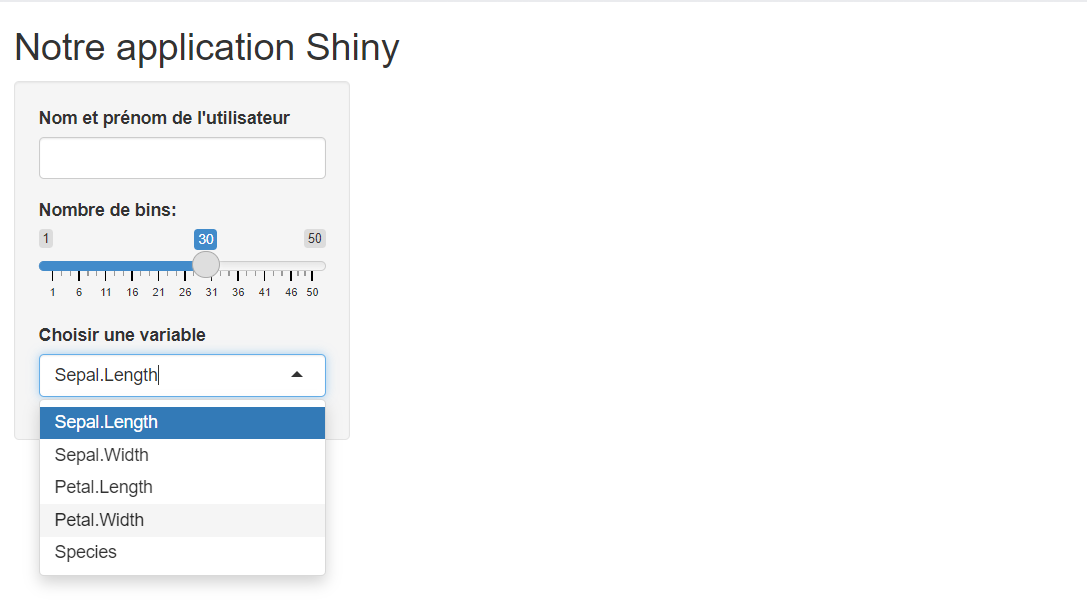
\includegraphics[keepaspectratio]{../images/input.png}}

Il existe une varieté d'inputs pour des actions spécifiques.

\pandocbounded{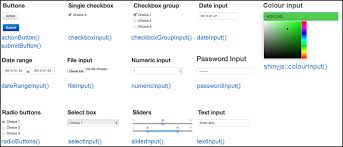
\includegraphics[keepaspectratio]{../images/typeinput.jpeg}}

\subsubsection{Outputs}\label{outputs}

Les \textbf{outputs} permettent de créer des \textbf{espaces réservés}
pour afficher les résultats générés par l'application dans le
\textbf{panneau principal}.

Ces sorties peuvent être de \textbf{n'importe quel type d'objet R} :
graphiques, tableaux, textes, résumés statistiques, etc.

Shiny propose différentes fonctions de sortie, chacune adaptée à un type
spécifique :

\begin{itemize}
\tightlist
\item
  \texttt{textOutput()} : pour afficher \textbf{du texte dynamique}.\\
\item
  \texttt{verbatimTextOutput()} : pour afficher \textbf{du texte brut}
  (résumé, message, structure\ldots).\\
\item
  \texttt{plotOutput()} : pour afficher \textbf{des graphiques}.\\
\item
  \texttt{DTOutput()} : pour afficher \textbf{des tableaux interactifs}
  avec le package \texttt{DT}.
\end{itemize}

Dans notre exemple, chaque sortie est placée dans un \textbf{onglet
distinct} pour une organisation claire et lisible.

\begin{Shaded}
\begin{Highlighting}[]
\FunctionTok{library}\NormalTok{(DT)}
\NormalTok{interface }\OtherTok{\textless{}{-}} \FunctionTok{fluidPage}\NormalTok{(}
  \FunctionTok{sidebarLayout}\NormalTok{(}
  \FunctionTok{sidebarPanel}\NormalTok{(),}
\FunctionTok{mainPanel}\NormalTok{ (}
 \FunctionTok{navlistPanel}\NormalTok{(}
    \FunctionTok{tabPanel}\NormalTok{(}\StringTok{"Nom et Prénom"}\NormalTok{,}\FunctionTok{textOutput}\NormalTok{(}\AttributeTok{outputId =} \StringTok{"name"}\NormalTok{)),}
    \FunctionTok{tabPanel}\NormalTok{(}\StringTok{"Visualisation des données"}\NormalTok{,}\FunctionTok{DTOutput}\NormalTok{(}\AttributeTok{outputId =} \StringTok{"iris\_data"}\NormalTok{)),}
    \FunctionTok{tabPanel}\NormalTok{(}\StringTok{"Statistiques"}\NormalTok{,}\FunctionTok{verbatimTextOutput}\NormalTok{(}\AttributeTok{outputId =} \StringTok{\textquotesingle{}summary\textquotesingle{}}\NormalTok{)),}
    \FunctionTok{tabPanel}\NormalTok{(}\StringTok{"Histogramme"}\NormalTok{,}\FunctionTok{plotOutput}\NormalTok{(}\AttributeTok{outputId =} \StringTok{\textquotesingle{}hist\textquotesingle{}}\NormalTok{))}
  
\NormalTok{      )}
\NormalTok{    )}
\NormalTok{  )}
\NormalTok{)}
\CommentTok{\# Run the application }
\FunctionTok{shinyApp}\NormalTok{(}\AttributeTok{ui =}\NormalTok{ interface, }\AttributeTok{server =}\NormalTok{ server)}
\end{Highlighting}
\end{Shaded}

Voici comment s'affichent nos différents onglets correspondants aux
outputs cités plus haut:

\pandocbounded{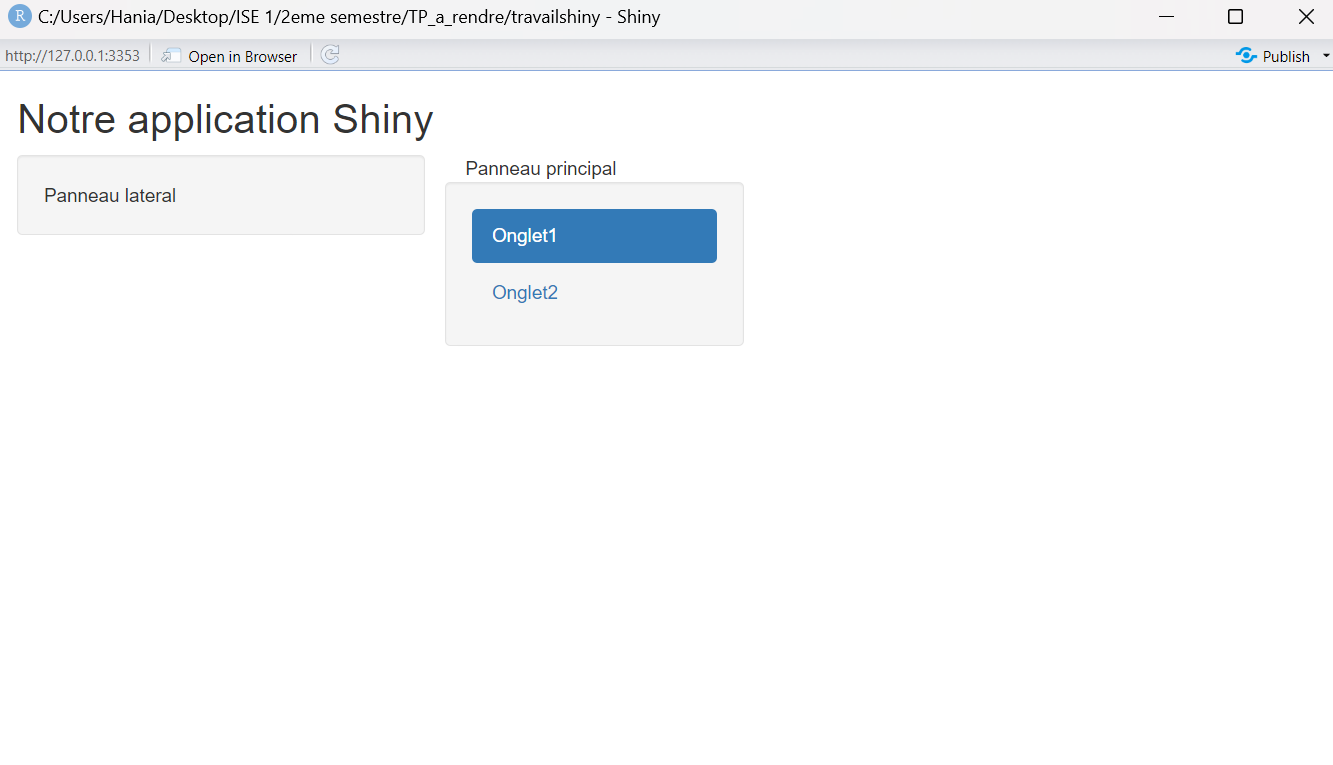
\includegraphics[keepaspectratio]{../images/output.png}}

Voici quelques outputs et leurs fonctions:

\begin{Shaded}
\begin{Highlighting}[]
\FunctionTok{library}\NormalTok{(knitr)}
\FunctionTok{kable}\NormalTok{(}
  \FunctionTok{data.frame}\NormalTok{(}
    \StringTok{"Type d’Output"} \OtherTok{=} \FunctionTok{c}\NormalTok{(}\StringTok{"Texte"}\NormalTok{, }\StringTok{"Texte HTML"}\NormalTok{, }\StringTok{"Tableau"}\NormalTok{, }\StringTok{"Tableau interactif"}\NormalTok{, }\StringTok{"Graphique de base"}\NormalTok{, }\StringTok{"Graphique interactif"}\NormalTok{, }\StringTok{"Texte/verbatim"}\NormalTok{, }\StringTok{"UI personnalisée"}\NormalTok{, }\StringTok{"Image"}\NormalTok{, }\StringTok{"Téléchargement"}\NormalTok{),}
    \StringTok{"Fonction UI"} \OtherTok{=} \FunctionTok{c}\NormalTok{(}\StringTok{"textOutput()"}\NormalTok{, }\StringTok{"htmlOutput()"}\NormalTok{, }\StringTok{"tableOutput()"}\NormalTok{, }\StringTok{"DT::dataTableOutput()"}\NormalTok{, }\StringTok{"plotOutput()"}\NormalTok{, }\StringTok{"plotlyOutput()"}\NormalTok{, }\StringTok{"verbatimTextOutput()"}\NormalTok{, }\StringTok{"uiOutput()"}\NormalTok{, }\StringTok{"imageOutput()"}\NormalTok{, }\StringTok{"downloadButton()"}\NormalTok{),}
    \StringTok{"Fonction server"} \OtherTok{=} \FunctionTok{c}\NormalTok{(}\StringTok{"renderText()"}\NormalTok{, }\StringTok{"renderUI()"}\NormalTok{, }\StringTok{"renderTable()"}\NormalTok{, }\StringTok{"DT::renderDataTable()"}\NormalTok{, }\StringTok{"renderPlot()"}\NormalTok{, }\StringTok{"renderPlotly()"}\NormalTok{, }\StringTok{"renderPrint()"}\NormalTok{, }\StringTok{"renderUI()"}\NormalTok{, }\StringTok{"renderImage()"}\NormalTok{, }\StringTok{"downloadHandler()"}\NormalTok{),}
    \StringTok{"Description"} \OtherTok{=} \FunctionTok{c}\NormalTok{(}
      \StringTok{"Affiche du texte brut dynamique"}\NormalTok{,}
      \StringTok{"Affiche du texte HTML formaté"}\NormalTok{,}
      \StringTok{"Affiche une table statique"}\NormalTok{,}
      \StringTok{"Tableau avec tri, recherche, pagination"}\NormalTok{,}
      \StringTok{"Graphique statique (base R ou ggplot2)"}\NormalTok{,}
      \StringTok{"Graphique interactif (zoom, survol)"}\NormalTok{,}
      \StringTok{"Affiche du texte brut (résultats de code)"}\NormalTok{,}
      \StringTok{"Interface générée dynamiquement"}\NormalTok{,}
      \StringTok{"Affiche une image"}\NormalTok{,}
      \StringTok{"Téléchargement de fichier"}
\NormalTok{    )}
\NormalTok{  ),}
  \AttributeTok{format =} \StringTok{"markdown"}\NormalTok{,}
  \AttributeTok{align =} \StringTok{"l"}
\NormalTok{)}
\end{Highlighting}
\end{Shaded}

\begin{longtable}[]{@{}
  >{\raggedright\arraybackslash}p{(\linewidth - 6\tabcolsep) * \real{0.1963}}
  >{\raggedright\arraybackslash}p{(\linewidth - 6\tabcolsep) * \real{0.2056}}
  >{\raggedright\arraybackslash}p{(\linewidth - 6\tabcolsep) * \real{0.2056}}
  >{\raggedright\arraybackslash}p{(\linewidth - 6\tabcolsep) * \real{0.3925}}@{}}
\toprule\noalign{}
\begin{minipage}[b]{\linewidth}\raggedright
Type.d.Output
\end{minipage} & \begin{minipage}[b]{\linewidth}\raggedright
Fonction.UI
\end{minipage} & \begin{minipage}[b]{\linewidth}\raggedright
Fonction.server
\end{minipage} & \begin{minipage}[b]{\linewidth}\raggedright
Description
\end{minipage} \\
\midrule\noalign{}
\endhead
\bottomrule\noalign{}
\endlastfoot
Texte & textOutput() & renderText() & Affiche du texte brut dynamique \\
Texte HTML & htmlOutput() & renderUI() & Affiche du texte HTML
formaté \\
Tableau & tableOutput() & renderTable() & Affiche une table statique \\
Tableau interactif & DT::dataTableOutput() & DT::renderDataTable() &
Tableau avec tri, recherche, pagination \\
Graphique de base & plotOutput() & renderPlot() & Graphique statique
(base R ou ggplot2) \\
Graphique interactif & plotlyOutput() & renderPlotly() & Graphique
interactif (zoom, survol) \\
Texte/verbatim & verbatimTextOutput() & renderPrint() & Affiche du texte
brut (résultats de code) \\
UI personnalisée & uiOutput() & renderUI() & Interface générée
dynamiquement \\
Image & imageOutput() & renderImage() & Affiche une image \\
Téléchargement & downloadButton() & downloadHandler() & Téléchargement
de fichier \\
\end{longtable}

\subsubsection{Quelques précisions sur les
outputs}\label{quelques-pruxe9cisions-sur-les-outputs}

Tout comme les fonctions d'input, les fonctions d'\textbf{output}
possèdent un argument essentiel : \textbf{\texttt{outputId}}, qui doit
être \textbf{unique} pour chaque sortie.

Ce \textbf{\texttt{outputId}} joue un rôle crucial : il permet au
\textbf{serveur} d'associer un contenu (graphique, texte, tableau\ldots)
à l'espace de sortie défini dans l'interface. C'est pourquoi son
\textbf{unicité} est indispensable.

\begin{quote}
\textbf{Important :} Jusqu'à présent, aucune sortie ne s'affiche
automatiquement dans l'application. C'est uniquement le \textbf{serveur}
qui déclenche leur génération et leur affichage en fonction des
instructions définies dans sa fonction.
\end{quote}

\subsection{Le serveur}\label{le-serveur}

Le \textbf{serveur} représente le \textbf{cœur logique} de l'application
Shiny. C'est lui qui traite les \textbf{interactions} de l'utilisateur
issues de l'interface (inputs) et qui génère les \textbf{sorties
dynamiques} (outputs) en réponse.

Pour cela, Shiny met à disposition plusieurs fonctions essentielles :

\begin{itemize}
\tightlist
\item
  \texttt{renderXXX()} : permet de \textbf{lier une sortie}
  (\texttt{outputId}) à une expression R (ex. : \texttt{renderPlot()},
  \texttt{renderText()}\ldots).\\
\item
  \texttt{reactive()} : crée des \textbf{objets réactifs}, qui se
  mettent automatiquement à jour lorsqu'un input change.\\
\item
  \texttt{observe()} : permet de \textbf{surveiller des changements}
  d'inputs et d'exécuter du code en conséquence (sans produire de sortie
  visible).
\end{itemize}

\subsubsection{\texorpdfstring{Les fonctions
\texttt{renderXXX()}}{Les fonctions renderXXX()}}\label{les-fonctions-renderxxx}

Dans le \textbf{serveur}, les fonctions \texttt{renderXXX()} servent à
\textbf{générer dynamiquement les contenus} affichés dans les zones
d'output définies dans l'interface utilisateur.

Chaque fonction \texttt{renderXXX()} correspond à une fonction
\texttt{XXXOutput()} utilisée dans l'UI. Par exemple :

\begin{itemize}
\tightlist
\item
  \texttt{renderPlot()} est lié à \texttt{plotOutput()} pour afficher un
  \textbf{graphique},\\
\item
  \texttt{renderText()} est lié à \texttt{textOutput()} pour afficher
  \textbf{du texte},\\
\item
  \texttt{renderDT()} est lié à \texttt{DTOutput()} pour afficher une
  \textbf{table interactive}.
\end{itemize}

Voici différentes fonctions \texttt{render()} et leurs fonctions :

\begin{longtable}[]{@{}
  >{\raggedright\arraybackslash}p{(\linewidth - 4\tabcolsep) * \real{0.2847}}
  >{\raggedright\arraybackslash}p{(\linewidth - 4\tabcolsep) * \real{0.2701}}
  >{\raggedright\arraybackslash}p{(\linewidth - 4\tabcolsep) * \real{0.4453}}@{}}
\toprule\noalign{}
\begin{minipage}[b]{\linewidth}\raggedright
Fonction \texttt{render()} côté \texttt{server}
\end{minipage} & \begin{minipage}[b]{\linewidth}\raggedright
Fonction \texttt{output} côté \texttt{ui}
\end{minipage} & \begin{minipage}[b]{\linewidth}\raggedright
Utilisation principale
\end{minipage} \\
\midrule\noalign{}
\endhead
\bottomrule\noalign{}
\endlastfoot
\texttt{renderText()} & \texttt{textOutput("id")} & Afficher du texte
dynamique (valeurs, résultats simples) \\
\texttt{renderPrint()} & \texttt{verbatimTextOutput("id")} & Afficher du
texte brut (résultat de code, résumés, etc.) \\
\texttt{renderTable()} & \texttt{tableOutput("id")} & Afficher un
tableau statique \\
\texttt{renderPlot()} & \texttt{plotOutput("id")} & Afficher un
graphique statique (R base, ggplot2, etc.) \\
\texttt{renderUI()} & \texttt{uiOutput("id")} ou
\texttt{htmlOutput("id")} & Générer dynamiquement une interface (textes,
boutons, etc.) \\
\texttt{renderImage()} & \texttt{imageOutput("id")} & Afficher une image
(locale ou générée) \\
\texttt{renderDataTable()} \emph{(package DT)} &
\texttt{dataTableOutput("id")} & Afficher un tableau interactif (tri,
recherche, etc.) \\
\texttt{renderPlotly()} \emph{(package plotly)} &
\texttt{plotlyOutput("id")} & Afficher un graphique interactif (zoom,
survol, etc.) \\
\end{longtable}

Ces fonctions exécutent du \textbf{code R} chaque fois qu'un input
change, assurant une mise à jour réactive des sorties.

\begin{quote}
Dans l'exemple qui suit :\\
- \texttt{renderText()} permet d'afficher le \textbf{nom et prénom}
saisis,\\
- \texttt{renderDT()} affiche les \textbf{données filtrées d'Iris},\\
- \texttt{renderPlot()} génère un \textbf{histogramme interactif}.
\end{quote}

\begin{Shaded}
\begin{Highlighting}[]
\NormalTok{server }\OtherTok{\textless{}{-}} \ControlFlowTok{function}\NormalTok{(input, output) \{}
  \CommentTok{\#texte}
\NormalTok{  output}\SpecialCharTok{$}\NormalTok{name}\OtherTok{=}\FunctionTok{renderText}\NormalTok{(}\FunctionTok{paste0}\NormalTok{(}\StringTok{"Je m\textquotesingle{}appelle "}\NormalTok{ ,input}\SpecialCharTok{$}\NormalTok{text))}
\NormalTok{  output}\SpecialCharTok{$}\NormalTok{iris\_data}\OtherTok{=}\FunctionTok{renderDT}\NormalTok{(\{iris\})}
  \CommentTok{\#resumé statistiques}
\NormalTok{  output}\SpecialCharTok{$}\NormalTok{summary}\OtherTok{=}\FunctionTok{renderPrint}\NormalTok{(\{}
    \FunctionTok{summary}\NormalTok{(iris) \})}
  \CommentTok{\#Histogrammes}
\NormalTok{  output}\SpecialCharTok{$}\NormalTok{hist}\OtherTok{=}\FunctionTok{renderPlot}\NormalTok{(\{ }\FunctionTok{hist}\NormalTok{(iris[[input}\SpecialCharTok{$}\NormalTok{var]], }
\AttributeTok{breaks =} \FunctionTok{seq}\NormalTok{(}\FunctionTok{min}\NormalTok{(iris[[input}\SpecialCharTok{$}\NormalTok{var]]), }\FunctionTok{max}\NormalTok{(iris[[input}\SpecialCharTok{$}\NormalTok{var]]), }\AttributeTok{length.out =}\NormalTok{ input}\SpecialCharTok{$}\NormalTok{slider),}
\AttributeTok{main =} \FunctionTok{paste}\NormalTok{(}\StringTok{"Histogramme de"}\NormalTok{, input}\SpecialCharTok{$}\NormalTok{var),}
\AttributeTok{xlab =}\NormalTok{ input}\SpecialCharTok{$}\NormalTok{var,}
\AttributeTok{ylab =} \StringTok{"Fréquence"}\NormalTok{) \})}
\NormalTok{\}  }
\end{Highlighting}
\end{Shaded}

Sortie Texte :

\pandocbounded{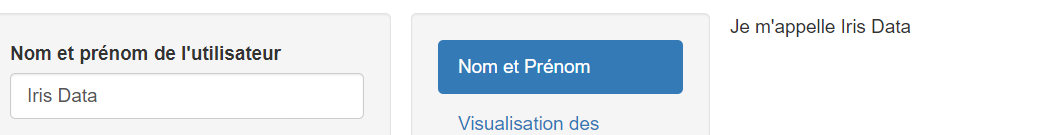
\includegraphics[keepaspectratio]{../images/renduTexte.png}}

Sortie Table :

\pandocbounded{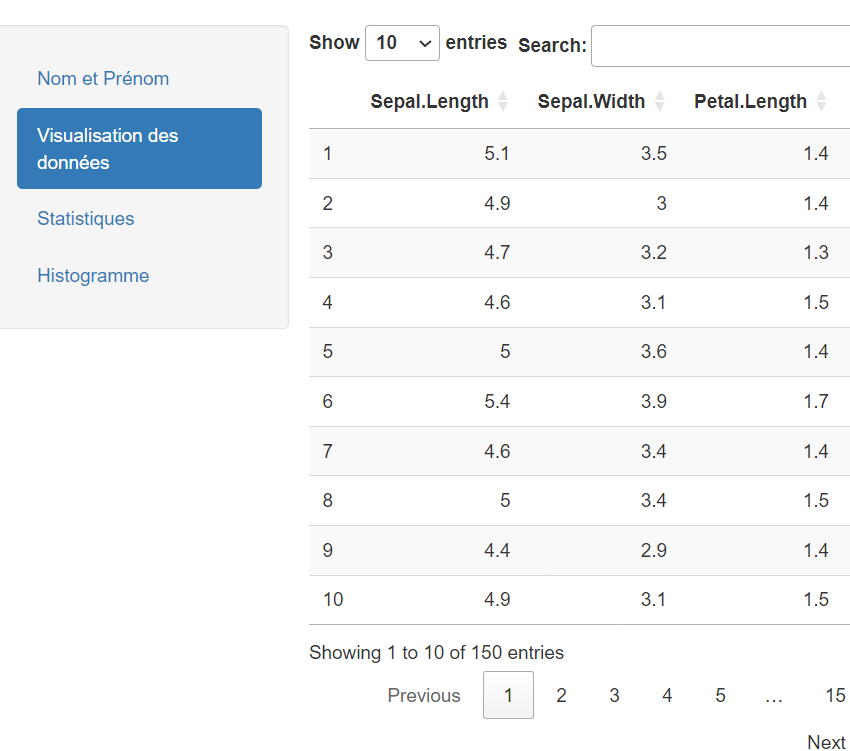
\includegraphics[keepaspectratio]{../images/renduTable.png}}

Sortie Statistiques :

\pandocbounded{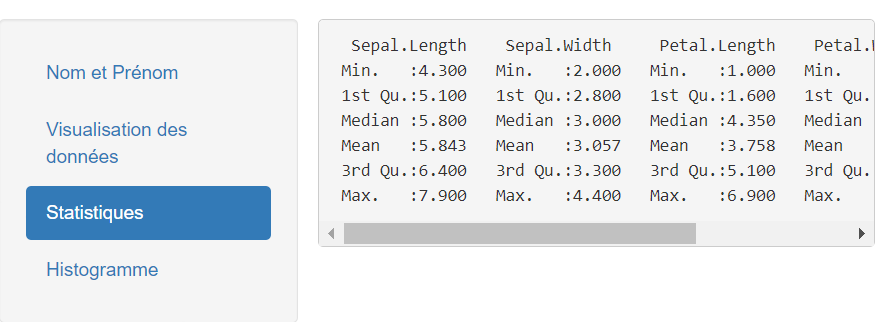
\includegraphics[keepaspectratio]{../images/renduStat.png}}

Sortie Histogramme :

\pandocbounded{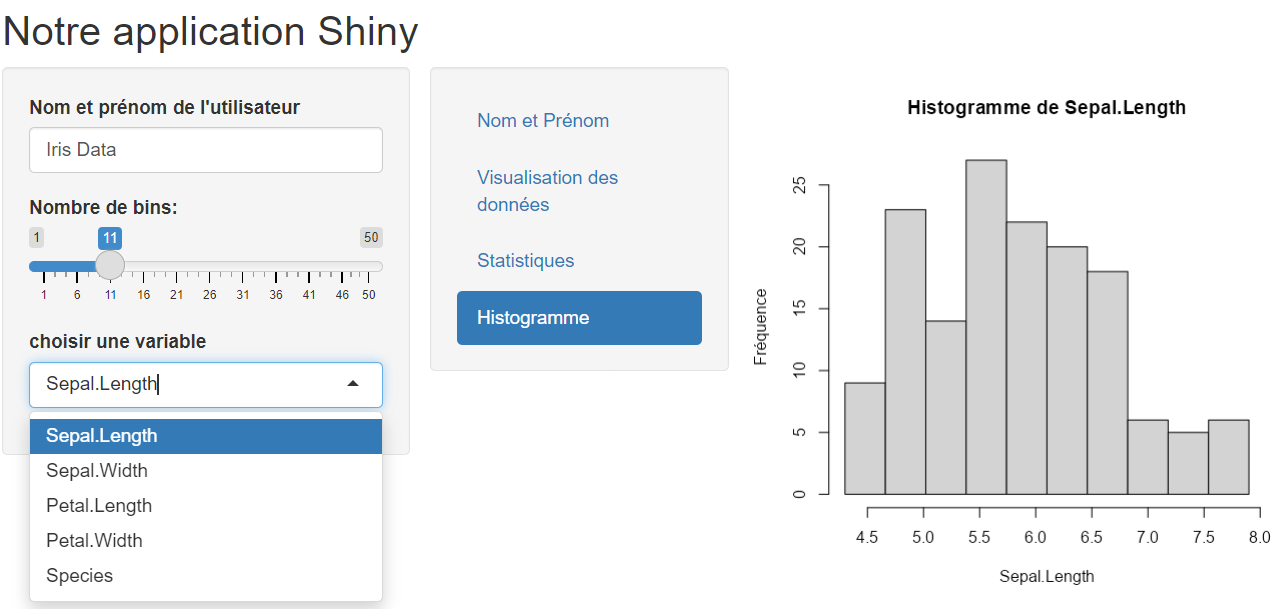
\includegraphics[keepaspectratio]{../images/renduHisto.png}}

\subsection{\texorpdfstring{La fonction
\texttt{reactive(\{\})}}{La fonction reactive(\{\})}}\label{la-fonction-reactive}

La \textbf{réactivité} est au cœur du fonctionnement des applications
Shiny. Elle permet à l'interface de se \textbf{mettre à jour
automatiquement} dès qu'un élément (input, donnée\ldots) change.

Dans ce contexte, la fonction \textbf{\texttt{reactive()}} (ou
\texttt{reactiveValues()}) est utilisée côté serveur pour créer des
\textbf{objets réactifs}. Ces objets :

\begin{itemize}
\tightlist
\item
  Sont recalculés \textbf{automatiquement} lorsque leurs dépendances
  changent,\\
\item
  Évitent les recalculs inutiles et facilitent la gestion des données
  dynamiques.
\end{itemize}

\begin{quote}
Les objets créés avec \texttt{reactive()} sont souvent utilisés à
l'intérieur des fonctions \texttt{renderXXX()} pour produire des sorties
actualisées en temps réel.
\end{quote}

\begin{Shaded}
\begin{Highlighting}[]
\FunctionTok{library}\NormalTok{(DT)}
\NormalTok{server }\OtherTok{\textless{}{-}} \ControlFlowTok{function}\NormalTok{(input, output, session) \{    }
\NormalTok{    df}\OtherTok{=}\FunctionTok{reactive}\NormalTok{(\{ }
\NormalTok{    iris}
\NormalTok{    \})}\CommentTok{\#Création de la variable reactive}
  
\NormalTok{  output}\SpecialCharTok{$}\NormalTok{iris\_data}\OtherTok{=}\FunctionTok{renderDT}\NormalTok{(\{}
    \FunctionTok{df}\NormalTok{() }\CommentTok{\#Utilisation de la variable dans une fonction render}
\NormalTok{  \})}
\NormalTok{\}}
\end{Highlighting}
\end{Shaded}

\subsubsection{Autres fonctions
réactives}\label{autres-fonctions-ruxe9actives}

En plus de \texttt{reactive()}, Shiny propose d'autres fonctions pour
gérer les interactions et la logique réactive :

\begin{itemize}
\tightlist
\item
  \textbf{\texttt{observeEvent()}} : déclenche une action
  \textbf{lorsqu'un événement spécifique} (comme un clic sur un bouton)
  se produit.\\
\item
  \textbf{\texttt{observe()}} : \textbf{surveille des expressions
  réactives}, mais \textbf{ne produit pas de sortie} visible. Utile pour
  exécuter des opérations comme des enregistrements ou envois
  d'alertes.\\
\item
  \textbf{\texttt{isolate()}} : permet d'\textbf{empêcher un recalcul
  automatique} en \textbf{brisant temporairement la réactivité}. Cela
  évite des mises à jour inutiles dans certains cas.
\end{itemize}

\newpage

\section{Amélioration de l'apparence d'une application
Shiny}\label{amuxe9lioration-de-lapparence-dune-application-shiny}

Améliorer l'apparence d'une application Shiny ne repose pas uniquement
sur la \textbf{structure} (panneaux, onglets, etc.), mais aussi sur le
\textbf{style visuel}, notamment à travers les \textbf{thèmes}.

\subsection{\texorpdfstring{Le package
\texttt{shinythemes}}{Le package shinythemes}}\label{le-package-shinythemes}

Le moyen le plus simple de personnaliser le style d'une application est
d'utiliser le package \textbf{\texttt{shinythemes}}, qui propose une
\textbf{large sélection de thèmes prédéfinis}.

Pour appliquer un thème, il suffit d'ajouter la fonction
\texttt{shinytheme("nom\_du\_thème")} dans l'UI.

\begin{quote}
Exemple : ici, nous utilisons le thème \texttt{"journal"} pour un rendu
\end{quote}

\begin{Shaded}
\begin{Highlighting}[]
\FunctionTok{library}\NormalTok{(shiny)}
\FunctionTok{library}\NormalTok{(shinythemes)}

\NormalTok{ui }\OtherTok{\textless{}{-}} \FunctionTok{fluidPage}\NormalTok{(}
  \AttributeTok{theme =} \FunctionTok{shinytheme}\NormalTok{(}\StringTok{"journal"}\NormalTok{),  }\CommentTok{\# Change le thème ici (ex : "cosmo", "darkly", "flatly")}
  \FunctionTok{titlePanel}\NormalTok{(}\StringTok{"Exemple de thème Shiny"}\NormalTok{),}
  \FunctionTok{sidebarLayout}\NormalTok{(}
    \FunctionTok{sidebarPanel}\NormalTok{(}
      \FunctionTok{helpText}\NormalTok{(}\StringTok{"Ceci est un panneau latéral."}\NormalTok{)}
\NormalTok{    ),}
    \FunctionTok{mainPanel}\NormalTok{(}
      \FunctionTok{h3}\NormalTok{(}\StringTok{"Contenu principal"}\NormalTok{),}
      \FunctionTok{textOutput}\NormalTok{(}\StringTok{"texte"}\NormalTok{)}
\NormalTok{    )}
\NormalTok{  )}
\NormalTok{)}

\NormalTok{server }\OtherTok{\textless{}{-}} \ControlFlowTok{function}\NormalTok{(input, output, session) \{}
\NormalTok{  output}\SpecialCharTok{$}\NormalTok{texte }\OtherTok{\textless{}{-}} \FunctionTok{renderText}\NormalTok{(\{}
    \StringTok{"Bienvenue dans l\textquotesingle{}application avec thème !"}
\NormalTok{  \})}
\NormalTok{\}}

\FunctionTok{shinyApp}\NormalTok{(ui, server)}
\end{Highlighting}
\end{Shaded}

\pandocbounded{
\includegraphics[keepaspectratio]{../images/journal.png}}

La liste de tous les thèmes disponibles se trouve sur le site
\textcolor{blue}{library(Bootswatch)}.

\subsection{Thème personnalisé avec un fichier
CSS}\label{thuxe8me-personnalisuxe9-avec-un-fichier-css}

Pour utiliser un \textbf{thème personnalisé} qui ne fait pas partie du
package \texttt{shinythemes}, il est possible d'ajouter un
\textbf{fichier CSS} à votre application.

\begin{enumerate}
\def\labelenumi{\arabic{enumi}.}
\tightlist
\item
  Créer un sous-dossier nommé \textbf{\texttt{www}} dans le répertoire
  de votre application Shiny.\\
\item
  Placer votre fichier \textbf{CSS} (par exemple \texttt{style.css})
  dans ce dossier.\\
\item
  Ajouter la ligne suivante dans la fonction \texttt{fluidPage()} de
  l'UI pour lier le fichier CSS :
\end{enumerate}

\begin{Shaded}
\begin{Highlighting}[]
\NormalTok{ui }\OtherTok{\textless{}{-}} \FunctionTok{fluidPage}\NormalTok{(}\AttributeTok{theme =} \StringTok{"theme.css"}\NormalTok{,}
                
\NormalTok{)}
\end{Highlighting}
\end{Shaded}

\textbf{NB :} Il est \textbf{essentiel} de placer le fichier CSS dans un
sous-dossier nommé \textbf{\texttt{www}}. C'est \textbf{la cause la plus
fréquente d'erreur} si le thème personnalisé ne s'affiche pas
correctement.

Shiny offre \textbf{de nombreuses possibilités} pour améliorer
l'interface et l'expérience utilisateur.\\
En plus des thèmes via \texttt{shinythemes} ou CSS, il existe des
\textbf{packages dédiés à la création d'interfaces avancées}, comme :

\begin{itemize}
\tightlist
\item
  \textbf{\texttt{shinydashboard}} : pour construire des tableaux de
  bord modernes avec des boîtes, des menus latéraux, des entêtes
  personnalisables, etc.
\end{itemize}

\newpage

\section{Shinydashboard}\label{shinydashboard}

Le package \textbf{\texttt{shinydashboard}} est une extension du package
\textbf{Shiny} qui permet de \textbf{concevoir des tableaux de bord
interactifs et visuellement attrayants} au sein d'applications web
développées avec R. Il fournit un ensemble de composants et d'outils
facilitant la création d'interfaces utilisateur structurées, avec une
disposition typique de tableau de bord (menus latéraux, en-têtes,
boîtes, onglets, etc.), adaptée à des analyses complexes et
interactives.

\subsection{Structure d'un dashboard}\label{structure-dun-dashboard}

Tout comme une application développée avec \textbf{Shiny}, une
application construite avec \textbf{Shinydashboard} se compose de trois
parties principales : l'\textbf{interface utilisateur} (\texttt{ui}), la
\textbf{partie serveur} (\texttt{server}) et la \textbf{commande
d'exécution} (\texttt{shinyApp()}).

La logique reste identique à celle d'une application Shiny classique :

\begin{itemize}
\tightlist
\item
  La \textbf{partie UI} définit la mise en page générale, les éléments
  visuels (menus, boîtes, graphiques, etc.) ainsi que les interactions
  avec l'utilisateur.
\item
  La \textbf{partie serveur} contient la logique de traitement,
  permettant de générer les résultats à afficher de manière dynamique.
\end{itemize}

Le package \textbf{shinydashboard} introduit cependant des fonctions
spécifiques comme \texttt{dashboardPage()}, \texttt{dashboardHeader()},
\texttt{dashboardSidebar()} et \texttt{dashboardBody()} pour structurer
l'interface selon un format de tableau de bord.

\subsection{Les principales
dispositions}\label{les-principales-dispositions}

Dans la partie \textbf{interface utilisateur}, la mise en page d'un
tableau de bord avec \textbf{shinydashboard} est gérée à l'aide de la
fonction \texttt{dashboardPage()}, qui organise l'interface en trois
zones principales :

\begin{itemize}
\tightlist
\item
  \texttt{dashboardHeader()} : définit l'en-tête de l'application (barre
  supérieure) ;
\item
  \texttt{dashboardSidebar()} : crée le panneau latéral, souvent utilisé
  pour la navigation ou les filtres ;
\item
  \texttt{dashboardBody()} : constitue la zone principale où s'affichent
  les contenus et résultats (graphiques, tableaux, etc.).
\end{itemize}

En plus de ces trois éléments essentiels, \texttt{dashboardPage()}
accepte des arguments optionnels comme :

\begin{itemize}
\tightlist
\item
  \texttt{title} : pour afficher un titre dans l'onglet du navigateur ;
\item
  \texttt{skin} : pour personnaliser le thème de couleur principal de
  l'application (par défaut : \textbf{bleu}, mais aussi disponible en
  \textbf{noir}, \textbf{rouge}, \textbf{jaune}, \textbf{vert},
  \textbf{violet}).
\end{itemize}

\begin{Shaded}
\begin{Highlighting}[]
\NormalTok{ui }\OtherTok{\textless{}{-}} \FunctionTok{dashboardPage}\NormalTok{(}
  \FunctionTok{dashboardHeader}\NormalTok{(}\AttributeTok{title=}\StringTok{"L\textquotesingle{}en{-}tete"}\NormalTok{),}
  \FunctionTok{dashboardSidebar}\NormalTok{(}\AttributeTok{title=}\StringTok{"Le panneau latéral "}\NormalTok{),}
  \FunctionTok{dashboardBody}\NormalTok{(}\StringTok{"Le panneau principal "}\NormalTok{),}
  \AttributeTok{skin=}\StringTok{"green"}
\NormalTok{)}
\NormalTok{server }\OtherTok{\textless{}{-}} \ControlFlowTok{function}\NormalTok{(input, output) \{}
\NormalTok{\}}
\FunctionTok{shinyApp}\NormalTok{(ui, server)}
\end{Highlighting}
\end{Shaded}

\pandocbounded{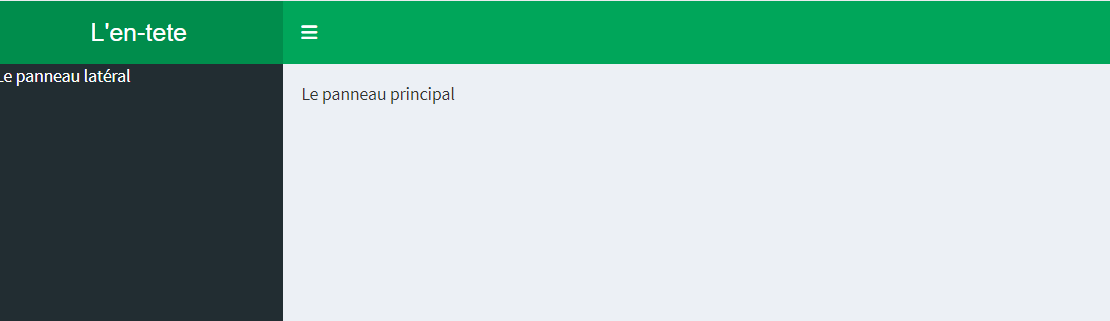
\includegraphics[keepaspectratio]{../images/entete.png}}

\subsection{Dispositions
supplémentaires}\label{dispositions-suppluxe9mentaires}

\subsubsection{Barre latérale}\label{barre-latuxe9rale}

La \textbf{barre latérale} (\texttt{dashboardSidebar()}) contient les
éléments permettant à l'utilisateur d'interagir avec la partie
principale de l'application ou de naviguer entre différentes sections.

On y retrouve à la fois :

\begin{itemize}
\tightlist
\item
  des \textbf{éléments d'entrée classiques} (\texttt{sliderInput()},
  \texttt{selectInput()}, etc.) ;
\item
  des \textbf{menus de navigation}, sous forme d'onglets, créés avec la
  fonction \texttt{menuItem()}.
\end{itemize}

Chaque \texttt{menuItem()} déclaré dans le \texttt{dashboardSidebar()}
correspond à un \texttt{tabItem()} défini dans le
\texttt{dashboardBody()}. La liaison entre ces deux éléments se fait via
l'argument \texttt{tabName}, qui doit être \textbf{identique et unique}
de part et d'autre.

\begin{Shaded}
\begin{Highlighting}[]
\FunctionTok{library}\NormalTok{(shiny)}
\FunctionTok{library}\NormalTok{(shinydashboard)}

\NormalTok{ui }\OtherTok{\textless{}{-}} \FunctionTok{dashboardPage}\NormalTok{(}
  \AttributeTok{skin=}\StringTok{"green"}\NormalTok{,}
  \FunctionTok{dashboardHeader}\NormalTok{(}\AttributeTok{title =} \StringTok{"Exemple d\textquotesingle{}Onglets"}\NormalTok{),}
  \FunctionTok{dashboardSidebar}\NormalTok{(}
    \FunctionTok{sidebarMenu}\NormalTok{(}
      \FunctionTok{menuItem}\NormalTok{(}\StringTok{"Dashboard"}\NormalTok{, }\AttributeTok{tabName =} \StringTok{"dashboard"}\NormalTok{, }\AttributeTok{icon =} \FunctionTok{icon}\NormalTok{(}\StringTok{"dashboard"}\NormalTok{)),}
      \FunctionTok{menuItem}\NormalTok{(}\StringTok{"Onglets"}\NormalTok{, }\AttributeTok{icon =} \FunctionTok{icon}\NormalTok{(}\StringTok{"th"}\NormalTok{), }\AttributeTok{tabName =} \StringTok{"widgets"}\NormalTok{,}
               \AttributeTok{badgeLabel =} \StringTok{"new"}\NormalTok{, }\AttributeTok{badgeColor =} \StringTok{"green"}\NormalTok{)}
\NormalTok{    )}
\NormalTok{  ),}
  \FunctionTok{dashboardBody}\NormalTok{(}
    \FunctionTok{tabItems}\NormalTok{(}
      \FunctionTok{tabItem}\NormalTok{(}\AttributeTok{tabName =} \StringTok{"dashboard"}\NormalTok{,}
        \FunctionTok{h2}\NormalTok{(}\StringTok{"Contenu du Dashboard"}\NormalTok{)}
\NormalTok{      ),}
      \FunctionTok{tabItem}\NormalTok{(}\AttributeTok{tabName =} \StringTok{"widgets"}\NormalTok{,}
        \FunctionTok{h2}\NormalTok{(}\StringTok{"Contenu des Onglets"}\NormalTok{)}
\NormalTok{      )}
\NormalTok{    )}
\NormalTok{  )}
\NormalTok{)}

\NormalTok{server }\OtherTok{\textless{}{-}} \ControlFlowTok{function}\NormalTok{(input, output, session) \{\}}

\FunctionTok{shinyApp}\NormalTok{(ui, server)}
\end{Highlighting}
\end{Shaded}

\pandocbounded{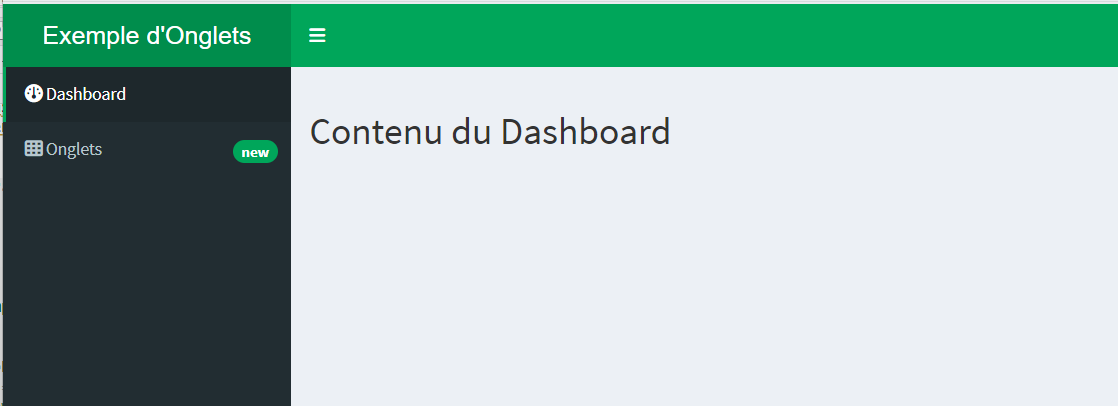
\includegraphics[keepaspectratio]{../images/barre.png}}

\subsubsection{Corps ou partie principale
:}\label{corps-ou-partie-principale}

Mis à part les \texttt{tabItem},la partie principale peut contenir
n'importe quel contenu standard de shiny mais, il est en plus possible
de déclarer des box pouvant inclure différents types de contenus, ce qui
est plus esthétique pour les tableaux de bord.

Cela se fait avec la fonction \texttt{box()}dans laquelle on peut
integrer des éléments de type input ou output.

Il en existe trois autres types :
\texttt{infoBox()},\texttt{valueBox},\texttt{tabBox()}.

La disposition des boites se fait avec \texttt{fluidrow()}ou
\texttt{column()}.

L'exemple suivant montre la création de differents types de box avec
affichages d'icônes issues de la bibliothèque \textbf{Font Awesome}, et
intégration des onglets pour le type tabBox.

\begin{Shaded}
\begin{Highlighting}[]
\FunctionTok{library}\NormalTok{(shiny)}
\FunctionTok{library}\NormalTok{(shinydashboard)}

\NormalTok{ui }\OtherTok{\textless{}{-}} \FunctionTok{dashboardPage}\NormalTok{(}
  \AttributeTok{skin=}\StringTok{"green"}\NormalTok{,}
  \FunctionTok{dashboardHeader}\NormalTok{(}\AttributeTok{title =} \StringTok{"Exemple de Boîtes"}\NormalTok{),}
  \FunctionTok{dashboardSidebar}\NormalTok{(),}
  \FunctionTok{dashboardBody}\NormalTok{(}
    \FunctionTok{fluidRow}\NormalTok{(}
      \CommentTok{\# InfoBox}
      \FunctionTok{infoBox}\NormalTok{(}\StringTok{"Nouvelles Notifications"}\NormalTok{, }\DecValTok{15}\NormalTok{, }\AttributeTok{icon =} \FunctionTok{icon}\NormalTok{(}\StringTok{"bell"}\NormalTok{), }\AttributeTok{color =} \StringTok{"blue"}\NormalTok{),}
      
      \CommentTok{\# ValueBox}
      \FunctionTok{valueBox}\NormalTok{(}\DecValTok{123}\NormalTok{, }\StringTok{"Utilisateurs actifs"}\NormalTok{, }\AttributeTok{icon =} \FunctionTok{icon}\NormalTok{(}\StringTok{"users"}\NormalTok{), }\AttributeTok{color =} \StringTok{"green"}\NormalTok{),}
      
      \CommentTok{\# Box avec onglets (TabBox)}
      \FunctionTok{tabBox}\NormalTok{(}
        \AttributeTok{title =} \StringTok{"Onglets Exemple"}\NormalTok{, }
        \FunctionTok{tabPanel}\NormalTok{(}\StringTok{"Tab1"}\NormalTok{, }\StringTok{"Contenu du premier onglet"}\NormalTok{),}
        \FunctionTok{tabPanel}\NormalTok{(}\StringTok{"Tab2"}\NormalTok{, }\StringTok{"Contenu du deuxième onglet"}\NormalTok{),}
        \FunctionTok{tabPanel}\NormalTok{(}\StringTok{"Tab3"}\NormalTok{, }\StringTok{"Contenu du troisième onglet"}\NormalTok{)}
\NormalTok{      )}
\NormalTok{    )}
\NormalTok{  )}
\NormalTok{)}

\NormalTok{server }\OtherTok{\textless{}{-}} \ControlFlowTok{function}\NormalTok{(input, output, session) \{\}}

\FunctionTok{shinyApp}\NormalTok{(ui, server)}
\end{Highlighting}
\end{Shaded}

\pandocbounded{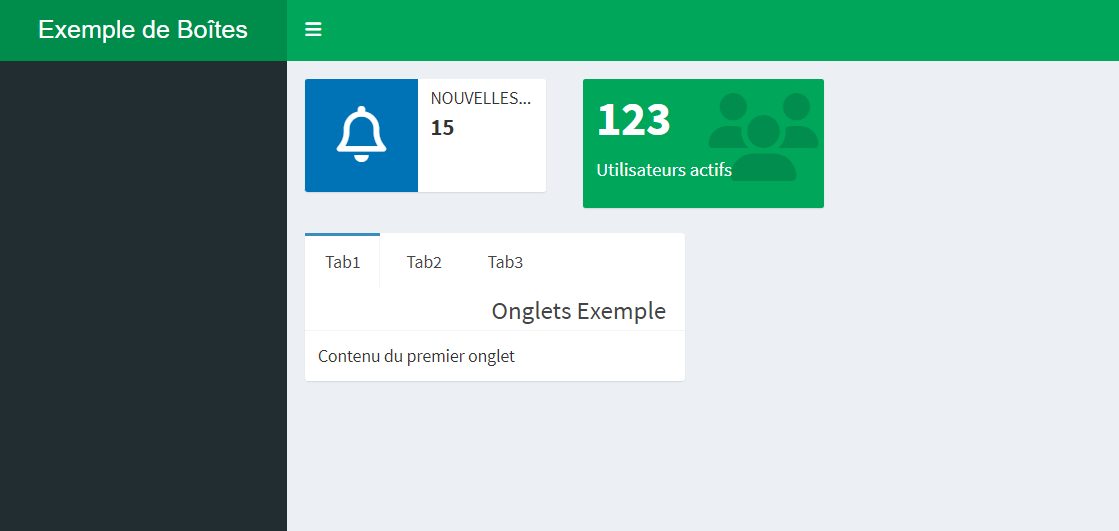
\includegraphics[keepaspectratio]{../images/corps_dash.png}}

\subsubsection{Le server}\label{le-server}

Dans une application \textbf{ShinyDashboard}, le \textbf{serveur}
conserve toutes les fonctions classiques de Shiny, telles que
\texttt{render()}, \texttt{output()}, \texttt{reactive()},
\texttt{observe()}, etc. Ces fonctions sont cruciales pour définir le
comportement interactif de l'application, traiter les données, générer
des sorties et maintenir la réactivité de l'interface utilisateur.

Dans la partie \textbf{UI} de l'application, les éléments de contenu,
tels que les onglets et les boîtes du tableau de bord, sont définis avec
des fonctions comme \texttt{tabItem()} ou \texttt{box()}. C'est ici que
l'on spécifie les sorties que l'on souhaite afficher (graphiques,
tableaux, valeurs, etc.) en utilisant des fonctions de sortie telles que
\textbf{\texttt{plotOutput()}, \texttt{tableOutput()},
\texttt{verbatimTextOutput()}}, et d'autres.

Côté \textbf{serveur}, des fonctions de rendu comme
\texttt{renderPlot()}, \texttt{renderTable()}, \texttt{renderText()},
etc., sont utilisées pour générer les sorties spécifiées dans la partie
UI.

En ce qui concerne la \textbf{réactivité}, chaque fois qu'il y a un
changement dans les entrées réactives utilisées pour générer les
sorties, le serveur est automatiquement déclenché pour recalculer et
mettre à jour les résultats associés. Cela se fait notamment grâce à
l'utilisation de \textbf{\texttt{observe()}} ou
\textbf{\texttt{reactive()}}. Ce mécanisme garantit que l'interface
utilisateur reste dynamique et que les contenus des
\textbf{\texttt{tabItem}} ou \textbf{\texttt{box}} sont continuellement
mis à jour en fonction des actions de l'utilisateur ou des modifications
des données.

\subsection{Exemple d'une application simple avec shinydashboard
utilisant les éléments vus
précédemment}\label{exemple-dune-application-simple-avec-shinydashboard-utilisant-les-uxe9luxe9ments-vus-pruxe9cuxe9demment}

\begin{Shaded}
\begin{Highlighting}[]
\NormalTok{data }\OtherTok{\textless{}{-}} \FunctionTok{data.frame}\NormalTok{(}
  \AttributeTok{x =} \DecValTok{1}\SpecialCharTok{:}\DecValTok{100}\NormalTok{,}
  \AttributeTok{y =} \FunctionTok{rnorm}\NormalTok{(}\DecValTok{100}\NormalTok{)}
\NormalTok{)}

\NormalTok{ui }\OtherTok{\textless{}{-}} \FunctionTok{dashboardPage}\NormalTok{(}
  \AttributeTok{skin=}\StringTok{"green"}\NormalTok{,}
  \FunctionTok{dashboardHeader}\NormalTok{(}\AttributeTok{title =} \StringTok{"Exemple de Tableau de Bord"}\NormalTok{, }\AttributeTok{titleWidth =} \DecValTok{450}\NormalTok{),}
  \FunctionTok{dashboardSidebar}\NormalTok{(}
    \FunctionTok{sidebarMenu}\NormalTok{(}
      \FunctionTok{menuItem}\NormalTok{(}\StringTok{"Onglet 1"}\NormalTok{, }\AttributeTok{tabName =} \StringTok{"tab1"}\NormalTok{),}
      \FunctionTok{menuItem}\NormalTok{(}\StringTok{"Onglet 2"}\NormalTok{, }\AttributeTok{tabName =} \StringTok{"tab2"}\NormalTok{)}
\NormalTok{    )}
\NormalTok{  ),}
  \FunctionTok{dashboardBody}\NormalTok{(}
    \FunctionTok{tabItems}\NormalTok{(}
      \FunctionTok{tabItem}\NormalTok{(}\AttributeTok{tabName =} \StringTok{"tab1"}\NormalTok{,}
              \FunctionTok{tabBox}\NormalTok{(}
                \AttributeTok{title =} \StringTok{"Tab Box 1"}\NormalTok{,}
                \FunctionTok{tabPanel}\NormalTok{(}\StringTok{"Graphique"}\NormalTok{, }\FunctionTok{plotOutput}\NormalTok{(}\StringTok{"plot1"}\NormalTok{)),}
                \FunctionTok{tabPanel}\NormalTok{(}\StringTok{"Tableau"}\NormalTok{, }\FunctionTok{tableOutput}\NormalTok{(}\StringTok{"table1"}\NormalTok{))}
\NormalTok{              ),}
              \FunctionTok{infoBox}\NormalTok{(}
                \StringTok{"Info Box"}\NormalTok{, }
                \StringTok{"Données générées aléatoirement"}\NormalTok{, }
                \AttributeTok{icon =} \FunctionTok{icon}\NormalTok{(}\StringTok{"info{-}circle"}\NormalTok{),}
                \AttributeTok{color =} \StringTok{"blue"}
\NormalTok{              ),}
              \FunctionTok{valueBox}\NormalTok{(}
                \FunctionTok{mean}\NormalTok{(data}\SpecialCharTok{$}\NormalTok{x),}
                \StringTok{"Moyenne de la variable x"}\NormalTok{,}
                \AttributeTok{icon =} \FunctionTok{icon}\NormalTok{(}\StringTok{"star"}\NormalTok{),}
                \AttributeTok{color =} \StringTok{"green"}
\NormalTok{              )}
\NormalTok{      ),}
      \FunctionTok{tabItem}\NormalTok{(}\AttributeTok{tabName =} \StringTok{"tab2"}\NormalTok{,}
              \FunctionTok{tabBox}\NormalTok{(}
                \AttributeTok{title =} \StringTok{"Tab Box 2"}\NormalTok{,}
                \FunctionTok{tabPanel}\NormalTok{(}\StringTok{"Graphique"}\NormalTok{, }\FunctionTok{plotOutput}\NormalTok{(}\StringTok{"plot2"}\NormalTok{))}
\NormalTok{              )}
\NormalTok{      )}
\NormalTok{    )}
\NormalTok{  )}
\NormalTok{)}

\NormalTok{server }\OtherTok{\textless{}{-}} \ControlFlowTok{function}\NormalTok{(input, output) \{}
\NormalTok{  output}\SpecialCharTok{$}\NormalTok{plot1 }\OtherTok{\textless{}{-}} \FunctionTok{renderPlot}\NormalTok{(\{}
    \FunctionTok{plot}\NormalTok{(data}\SpecialCharTok{$}\NormalTok{x, data}\SpecialCharTok{$}\NormalTok{y, }\AttributeTok{main =} \StringTok{"Graphique 1"}\NormalTok{, }\AttributeTok{type =} \StringTok{"l"}\NormalTok{, }\AttributeTok{col =} \StringTok{"blue"}\NormalTok{)}
\NormalTok{  \})}
\NormalTok{  output}\SpecialCharTok{$}\NormalTok{table1 }\OtherTok{\textless{}{-}} \FunctionTok{renderTable}\NormalTok{(\{}
    \FunctionTok{head}\NormalTok{(data)}
\NormalTok{  \})}
\NormalTok{  output}\SpecialCharTok{$}\NormalTok{plot2 }\OtherTok{\textless{}{-}} \FunctionTok{renderPlot}\NormalTok{(\{}
    \FunctionTok{plot}\NormalTok{(data}\SpecialCharTok{$}\NormalTok{y, data}\SpecialCharTok{$}\NormalTok{x, }\AttributeTok{main =} \StringTok{"Graphique 2"}\NormalTok{, }\AttributeTok{pch =} \DecValTok{19}\NormalTok{, }\AttributeTok{col =} \StringTok{"red"}\NormalTok{)}
\NormalTok{  \})}
\NormalTok{\}}

\FunctionTok{shinyApp}\NormalTok{(ui, server)}
\end{Highlighting}
\end{Shaded}

\pandocbounded{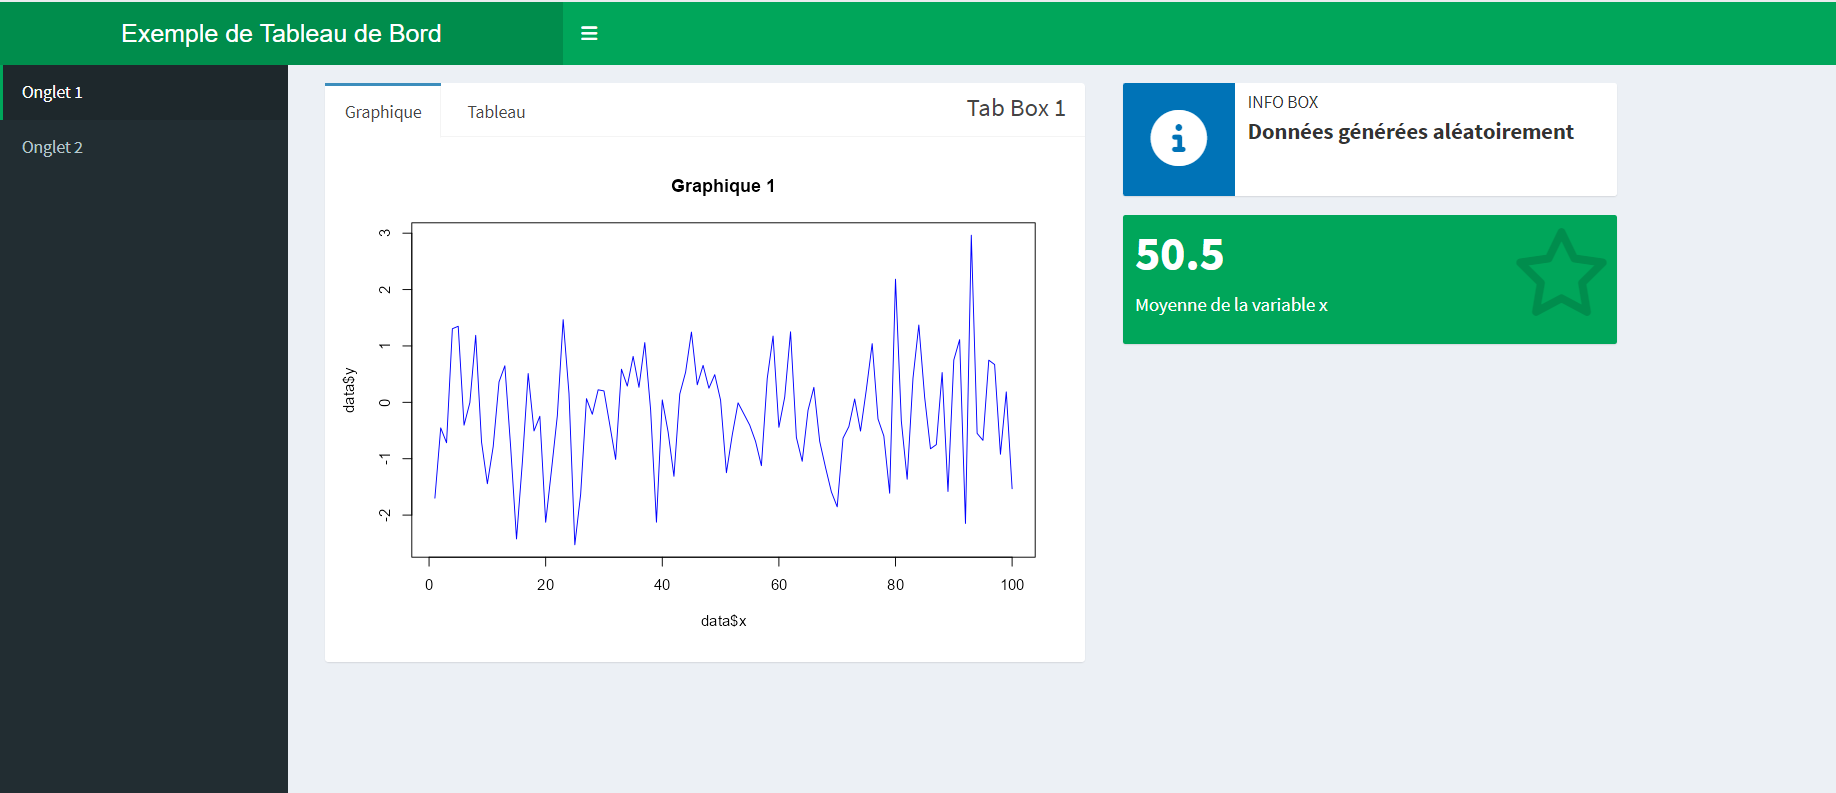
\includegraphics[keepaspectratio]{../images/All_parts.png}}

\newpage

\section{Publier une application
Shiny}\label{publier-une-application-shiny}

Lorsque l'on utilise la commande \texttt{runApp()}, R lance un petit
serveur Shiny local sur notre ordinateur, ce qui nous permet de
\textbf{tester l'application en local}. Cependant, cette méthode n'est
pas adaptée si l'on souhaite \textbf{partager l'application
publiquement} et la rendre accessible en ligne pour d'autres
utilisateurs.

\subsection{Hébergement sur shinyapp}\label{huxe9bergement-sur-shinyapp}

Il existe plusieurs façons de publier une application Shiny, et l'une
des plus simples consiste à utiliser le service
\href{https://www.shinyapps.io}{\textbf{shinyapps.io}}. Ce service
permet d'héberger gratuitement jusqu'à \textbf{5 applications par
utilisateur}.

Pour publier une application sur shinyapps.io, voici les étapes à suivre
:

\begin{enumerate}
\def\labelenumi{\arabic{enumi}.}
\item
  Créez un compte sur le site
  \href{https://www.shinyapps.io}{shinyapps.io} et connectez-vous.
\item
  Une fois connecté, vous accédez à un \textbf{tableau de bord} où
  seront listées vos applications. La première étape consiste à
  installer le package \textbf{\texttt{rsconnect}} dans R, qui vous
  permettra de déployer votre application directement depuis votre
  environnement R.
\end{enumerate}

\begin{Shaded}
\begin{Highlighting}[]
\FunctionTok{install.packages}\NormalTok{(}\StringTok{"rsconnect"}\NormalTok{)}
\end{Highlighting}
\end{Shaded}

\begin{enumerate}
\def\labelenumi{\arabic{enumi}.}
\setcounter{enumi}{2}
\tightlist
\item
  Ensuite, copier les lignes présentées dans la pop-up du type (ceci est
  un exemple avec le compte \emph{Jean-R-Shiny-2025}) :
\end{enumerate}

\begin{Shaded}
\begin{Highlighting}[]
\CommentTok{\#rsconnect::setAccountInfo(name=\textquotesingle{}Jean{-}R{-}Shiny{-}2025\textquotesingle{},}
                    \CommentTok{\#      token=\textquotesingle{}6280C86118286E5417298841A85EE625\textquotesingle{},}
                    \CommentTok{\#      secret=\textquotesingle{}ymUisnP7jRsyShTvGW0iAiUwnOGv98HnyMbcMd19\textquotesingle{})}
\end{Highlighting}
\end{Shaded}

\begin{enumerate}
\def\labelenumi{\arabic{enumi}.}
\setcounter{enumi}{3}
\item
  Exécuter ces lignes sous R : vous êtes alors connecté à votre compte
  shinyapps.io depuis R.
\item
  Il suffit maintenant d'exécuter la ligne de code suivante (mise en
  commentaire).
\end{enumerate}

\begin{Shaded}
\begin{Highlighting}[]
\CommentTok{\#rsconnect::deployApp("chemin\_vers\_le\_dossier\_de\_votre\_application")}
\end{Highlighting}
\end{Shaded}

\subsection{Mise en ligne de
l'application}\label{mise-en-ligne-de-lapplication}

Une fois votre application prête, elle peut être mise en ligne. Pour
cela, vous devez placer dans votre dossier de travail \textbf{soit un
fichier \texttt{app.R}}, soit \textbf{deux fichiers \texttt{ui.R} et
\texttt{server.R}}.

\textbf{Remarques importantes :}

\begin{itemize}
\item
  Si vous avez déjà un compte sur \textbf{shinyapps.io}, vous pouvez
  lancer la publication en cliquant sur \textbf{\emph{Publish
  Application\ldots{}}}, situé à droite du bouton \textbf{\emph{Run
  App}} dans RStudio.
\item
  RStudio vous demandera alors un \textbf{token} pour authentifier votre
  compte shinyapps.io. Il vous suffit de copier-coller ce token depuis
  votre compte shinyapps.io pour établir la connexion.
\item
  La publication peut prendre quelques minutes, car shinyapps.io
  installe automatiquement tous les packages nécessaires au
  fonctionnement de votre application sur son serveur.
\item
  Une fois l'opération terminée, votre application s'ouvrira
  automatiquement dans votre navigateur web.
\item
  Si vous perdez l'URL de votre application, pas de panique : vous
  pouvez retrouver toutes vos applications dans votre tableau de bord
  sur shinyapps.io.
\end{itemize}

\subsection{Mise à jour d'une application
Shiny}\label{mise-uxe0-jour-dune-application-shiny}

Pour mettre à jour votre application, il suffit simplement de relancer
la commande \textbf{\emph{Publish Application\ldots{}}}. L'ancienne
version sera alors automatiquement \textbf{remplacée par la nouvelle}.

\newpage

\textcolor{blue}{\section*{CONCLUSION}\addcontentsline{toc}{section}{CONCLUSION}}

\subsection{Conclusion}\label{conclusion}

R Shiny est un outil puissant et accessible pour créer des applications
web interactives avec R. Il permet de concevoir des interfaces
intuitives, de visualiser dynamiquement des données, et de partager des
analyses en ligne.

Grâce à sa large communauté, ses nombreux packages complémentaires et
ses possibilités d'extension, Shiny constitue une solution complète pour
répondre aux besoins en visualisation, recherche ou communication de
données.

Maîtriser Shiny représente donc un véritable atout pour tout
professionnel souhaitant valoriser et diffuser ses analyses de manière
interactive et professionnelle. \newpage

\textcolor{blue}{\section*{BIBLIOGRAPHIE et WEBOGRAPHIE}\addcontentsline{toc}{section}{BIBLIOGRAPHIE et WEBOGRAPHIE}}

\end{document}
